\documentclass[tikz,border=8pt]{standalone}
\usepackage[T1]{fontenc}
\usepackage{helvet}
\renewcommand{\familydefault}{\sfdefault}
\usepackage{xcolor}
\usepackage{amssymb}
\usetikzlibrary{calc,positioning,shadows.blur}

% ---------- Colors ----------
\definecolor{bg}{HTML}{F7F8F4}
\definecolor{ink}{HTML}{1F2A2E}
\definecolor{green}{HTML}{2F5D3A}
\definecolor{greenlight}{HTML}{EAF2EA}
\definecolor{blueN}{HTML}{1565C0}
\definecolor{redO}{HTML}{D32F2F}
\definecolor{softgray}{HTML}{D6DDD4}
\definecolor{gold}{HTML}{C99422}

% ---------- Styles ----------
\tikzset{
  molbond/.style={
    line width=1.15pt,
    draw=ink,
    line cap=round
  },
  natom/.style={
    font=\bfseries\LARGE,
    text=blueN,
    fill=bg,
    inner sep=1.4pt
  },
  oatom/.style={
    font=\bfseries\LARGE,
    text=redO,
    fill=bg,
    inner sep=1.4pt
  },
  methyl/.style={
    font=\Large,
    text=ink,
    fill=bg,
    inner sep=1.4pt
  },
  card/.style={
    rounded corners=12pt,
    draw=softgray,
    line width=0.8pt,
    fill=white,
    blur shadow={
      shadow blur steps=5,
      shadow xshift=0.6pt,
      shadow yshift=-0.8pt,
      shadow opacity=20
    }
  },
  passmark/.style={
    circle,
    draw=green,
    fill=greenlight,
    line width=0.8pt,
    minimum size=0.68cm,
    font=\bfseries\normalsize,
    text=green
  },
  smalltext/.style={
    font=\small,
    text=ink,
    align=center
  },
  valuetext/.style={
    font=\bfseries\Large,
    text=green,
    align=center
  },
  labeltext/.style={
    font=\bfseries\small,
    text=ink,
    align=center
  }
}

\begin{document}

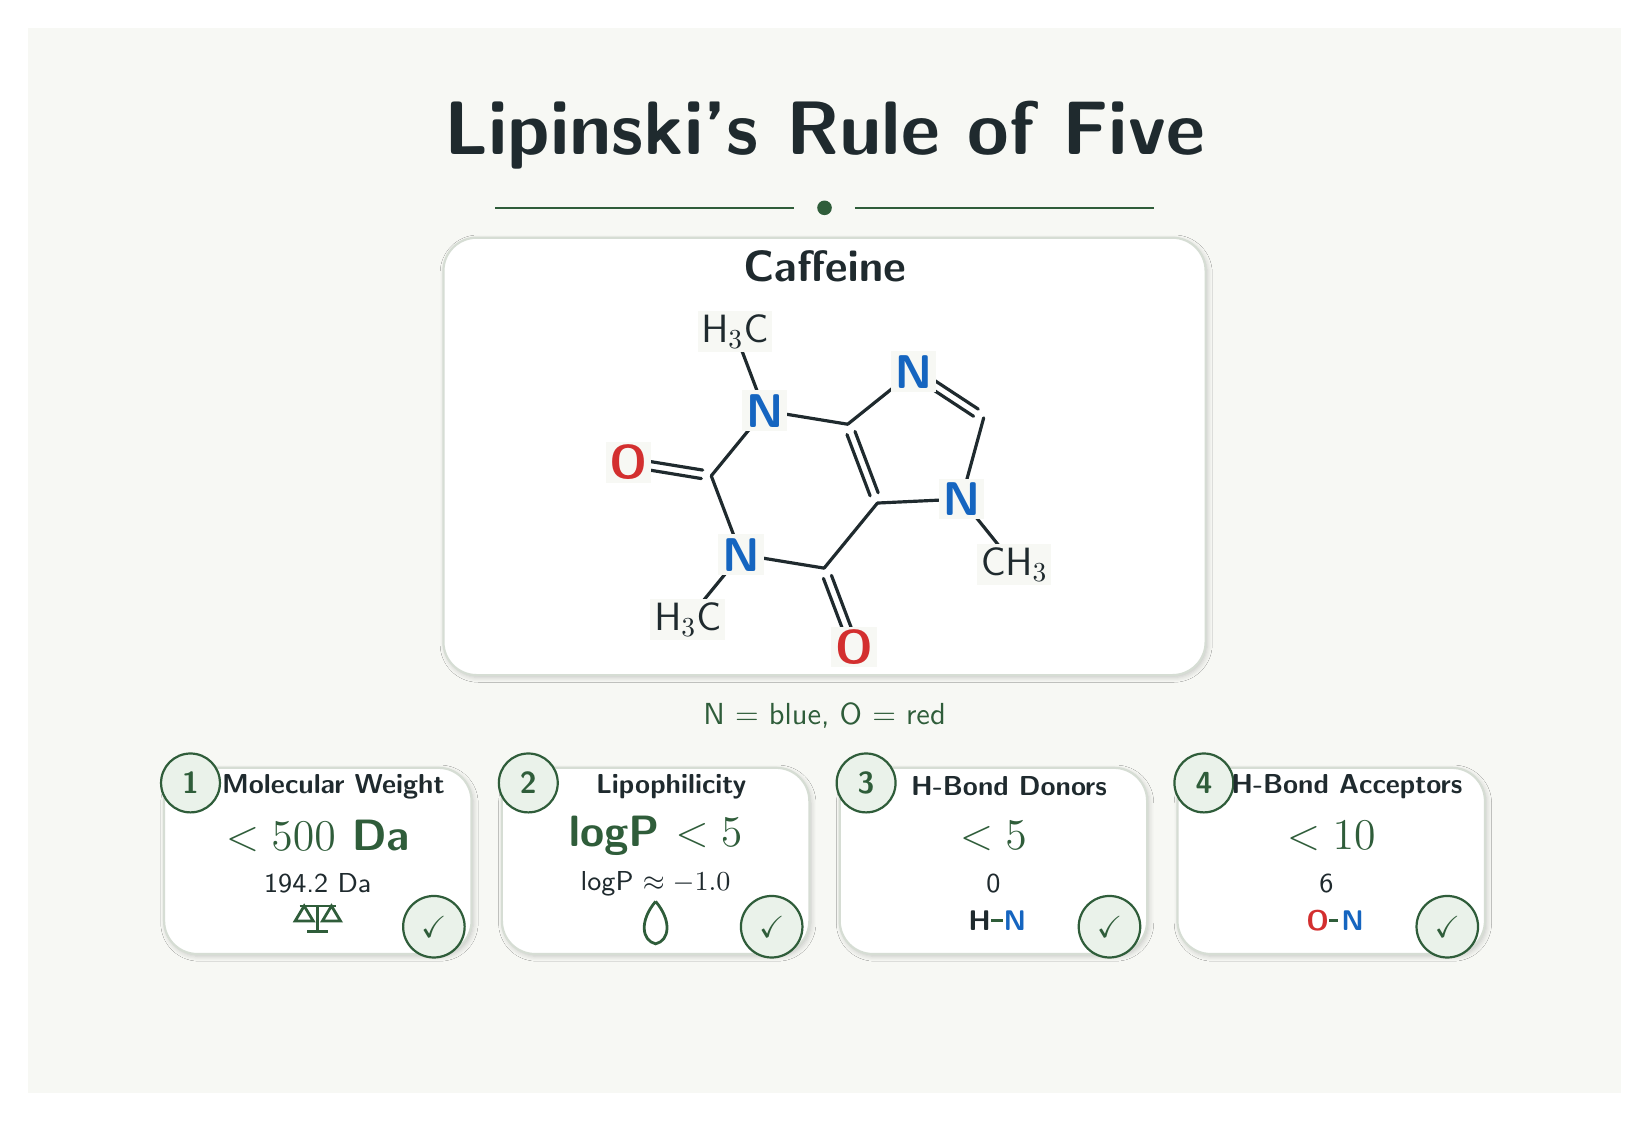
\begin{tikzpicture}[x=1cm,y=1cm, scale=1.10, transform shape]

% Background
\fill[bg] (-9.2,-6.4) rectangle (9.2,5.9);

% Title
\node[
  font=\bfseries\fontsize{32}{36}\selectfont,
  text=ink
] at (0,4.65)
  {Lipinski's Rule of Five};

\draw[green,line width=0.9pt] (-3.8,3.82) -- (-0.35,3.82);
\draw[green,line width=0.9pt] (0.35,3.82) -- (3.8,3.82);
\fill[green] (0,3.82) circle (2.4pt);

% Central molecule card
\node[card, minimum width=8.8cm, minimum height=5.05cm] at (0,0.95) {};

\node[
  font=\bfseries\Large,
  text=ink
] at (0,3.15) {Caffeine};

% Molecule generated from 2D coordinates, then redrawn in TikZ
\begin{scope}[shift={(0,0.57)}, scale=0.90]

% coordinates
\coordinate (a0) at (2.433,-0.967);
\coordinate (a1) at (1.757,-0.125);
\coordinate (a2) at (2.042,0.917);
\coordinate (a3) at (1.139,1.510);
\coordinate (a4) at (0.297,0.835);
\coordinate (a5) at (-0.769,1.009);
\coordinate (a6) at (-1.151,2.019);
\coordinate (a7) at (-1.453,0.173);
\coordinate (a8) at (-2.519,0.347);
\coordinate (a9) at (-1.071,-0.837);
\coordinate (a10) at (-1.755,-1.673);
\coordinate (a11) at (-0.005,-1.011);
\coordinate (a12) at (0.377,-2.022);
\coordinate (a13) at (0.679,-0.176);

% bonds
\draw[molbond] (a0) -- (a1);
\draw[molbond] (a1) -- (a2);
\draw[molbond] (1.912,0.937) -- (1.210,1.398);
\draw[molbond] (1.972,1.029) -- (1.270,1.490);
\draw[molbond] (a3) -- (a4);
\draw[molbond] (a4) -- (a5);
\draw[molbond] (a5) -- (a6);
\draw[molbond] (a5) -- (a7);
\draw[molbond] (-1.580,0.138) -- (-2.409,0.274);
\draw[molbond] (-1.563,0.247) -- (-2.392,0.382);
\draw[molbond] (a7) -- (a9);
\draw[molbond] (a9) -- (a10);
\draw[molbond] (a9) -- (a11);
\draw[molbond] (0.089,-1.104) -- (0.386,-1.890);
\draw[molbond] (-0.014,-1.143) -- (0.283,-1.929);
\draw[molbond] (a11) -- (a13);
\draw[molbond] (a13) -- (a1);
\draw[molbond] (0.585,-0.083) -- (0.288,0.703);
\draw[molbond] (0.688,-0.044) -- (0.391,0.742);

% atom labels
\node[methyl] at (a0) {CH$_3$};
\node[methyl] at (a6) {H$_3$C};
\node[methyl] at (a10) {H$_3$C};

\node[natom] at (a1) {N};
\node[natom] at (a3) {N};
\node[natom] at (a5) {N};
\node[natom] at (a9) {N};

\node[oatom] at (a8) {O};
\node[oatom] at (a12) {O};

\end{scope}

\node[font=\normalsize, text=green] at (0,-2.05) {N = blue, O = red};

% ---------- Rule cards ----------
\foreach \x/\num/\head/\rule/\value in {
  -5.85/1/Molecular Weight/$< 500$ Da/194.2 Da,
  -1.95/2/Lipophilicity/logP $< 5$/logP $\approx -1.0$,
   1.95/3/H-Bond Donors/$< 5$/0,
   5.85/4/H-Bond Acceptors/$< 10$/6
}{
  \node[card, minimum width=3.55cm, minimum height=2.15cm] at (\x,-3.72) {};
  \node[passmark] at ($ (\x,-2.82) + (-1.47,0) $) {\num};
  \node[labeltext] at ($ (\x,-2.86) + (0.18,0) $) {\head};
  \node[valuetext] at (\x,-3.43) {\rule};
  \node[smalltext] at (\x,-3.98) {\value};
  \node[passmark] at ($ (\x,-4.48) + (1.34,0) $) {\checkmark};
}

% ---------- Icons ----------

% molecular weight scale
\begin{scope}[shift={(-5.85,-4.45)}, scale=0.35]
\draw[green,line width=1pt] (-0.6,0.6)--(0.6,0.6);
\draw[green,line width=1pt] (0,0.6)--(0,-0.25);
\draw[green,line width=1pt] (-0.45,0.6)--(-0.75,0.1)--(-0.15,0.1)--cycle;
\draw[green,line width=1pt] (0.45,0.6)--(0.15,0.1)--(0.75,0.1)--cycle;
\draw[green,line width=1pt] (-0.35,-0.25)--(0.35,-0.25);
\end{scope}

% droplet
\begin{scope}[shift={(-1.95,-4.45)}, scale=0.35]
\draw[green,line width=1pt]
  (0,0.75)
  .. controls (-0.55,0.10) and (-0.45,-0.55) .. (0,-0.65)
  .. controls (0.45,-0.55) and (0.55,0.10) .. (0,0.75);
\end{scope}

% donor icon
\begin{scope}[shift={(1.95,-4.45)}, scale=0.45]
\node[text=ink,font=\bfseries\huge] at (-0.35,0.1) {H};
\draw[green,line width=1.2pt] (-0.05,0.1)--(0.25,0.1);
\node[text=blueN,font=\bfseries\huge] at (0.55,0.1) {N};
\end{scope}

% acceptor icon
\begin{scope}[shift={(5.85,-4.45)}, scale=0.45]
\node[text=redO,font=\bfseries\huge] at (-0.35,0.1) {O};
\draw[green,line width=1.2pt, dashed] (-0.05,0.1)--(0.25,0.1);
\node[text=blueN,font=\bfseries\huge] at (0.55,0.1) {N};
\end{scope}

\end{tikzpicture}

\end{document}

% pdflatex -interaction=nonstopmode -output-directory=synedu/S01/figure synedu/S01/figure/caffein.tex

% pdf2svg synedu/S01/figure/caffein.pdf docs/_static/images/talks/RO5.svg